% -*- TeX-master: "User_guide"; fill-column: 75 -*-

\section{Why are there differences?}
\label{sec:jsbml-design-goals}

In developing a pure Java Application Programming Interface (API) for
working with SBML, our intention was not to simply reimplement the Java API
already provided by libSBML~\citep{Bornstein2008}.
\index{application programming interface!libSBML}
We took the opportunity to rethink the API
\index{application programming interface!JSBML} from the ground up to
produce something more natural for Java programmers; moreover, we
benefited from being able to take a fresh look at today's entire set of
SBML specifications~\citep{Hucka2003, Hucka2008, Hucka2010a}
\index{SBML!specification} and redesign, for example, JSBML's type
hierarchy without the constraints of backwards compatibility that libSBML
faces. 

JSBML has also been developed as a library that provides more than only
facilities for reading, manipulating, and writing SBML files and data
streams. Although SBML only defines the structure of representations of
biological processes in files and does not prescribe how its components
should be stored \emph{in computer memory}, many software developers
nevertheless find it convenient to follow similar representational
structures in their programs. \index{model!storage and exchange} With this
in mind, we designed JSBML with the intention that it be directly usable as
a flexible internal data structure for numerical computation,
visualization, and more. With the help of its \emph{modules}, JSBML can
also be used as a communication layer between applications. For instance,
JSBML facilitates the implementation of plugins for
CellDesigner~\citep{Funahashi2003}, \index{CellDesigner} a popular software
application for modeling and simulation in systems biology. Finally, JSBML
(like libSBML before it) hides some of the differences and inconsistencies
in SBML \index{SBML!differences between Levels} that grew into the language
over the years as it evolved from Level to Level and Version to Version;
this makes it considerably easier for developers to support multiple
Levels/Versions of SBML transparently.

Where possible, we maintained many of libSBML's naming conventions for
methods and variables. Owing to the very different backgrounds of the two
libraries, and the fact that libSBML is implemented in C \index{C} and
C++ \index{C++}, some differences are unavoidable. To help libSBML
developers transition more easily to using JSBML, we provide a
compatibility module that implements many libSBML methods as adaptors
around the corresponding JSBML methods.

% FIXME add back somehow:
% during
% the evolution of SBML some elements or properties of elements have become
% obsolete.
% \index{deprecation}%


\section{Differences between the class hierarchies}
\label{sec:extended-type-hierarchy}

\begin{sidewaysfigure}[p]
  \centering
  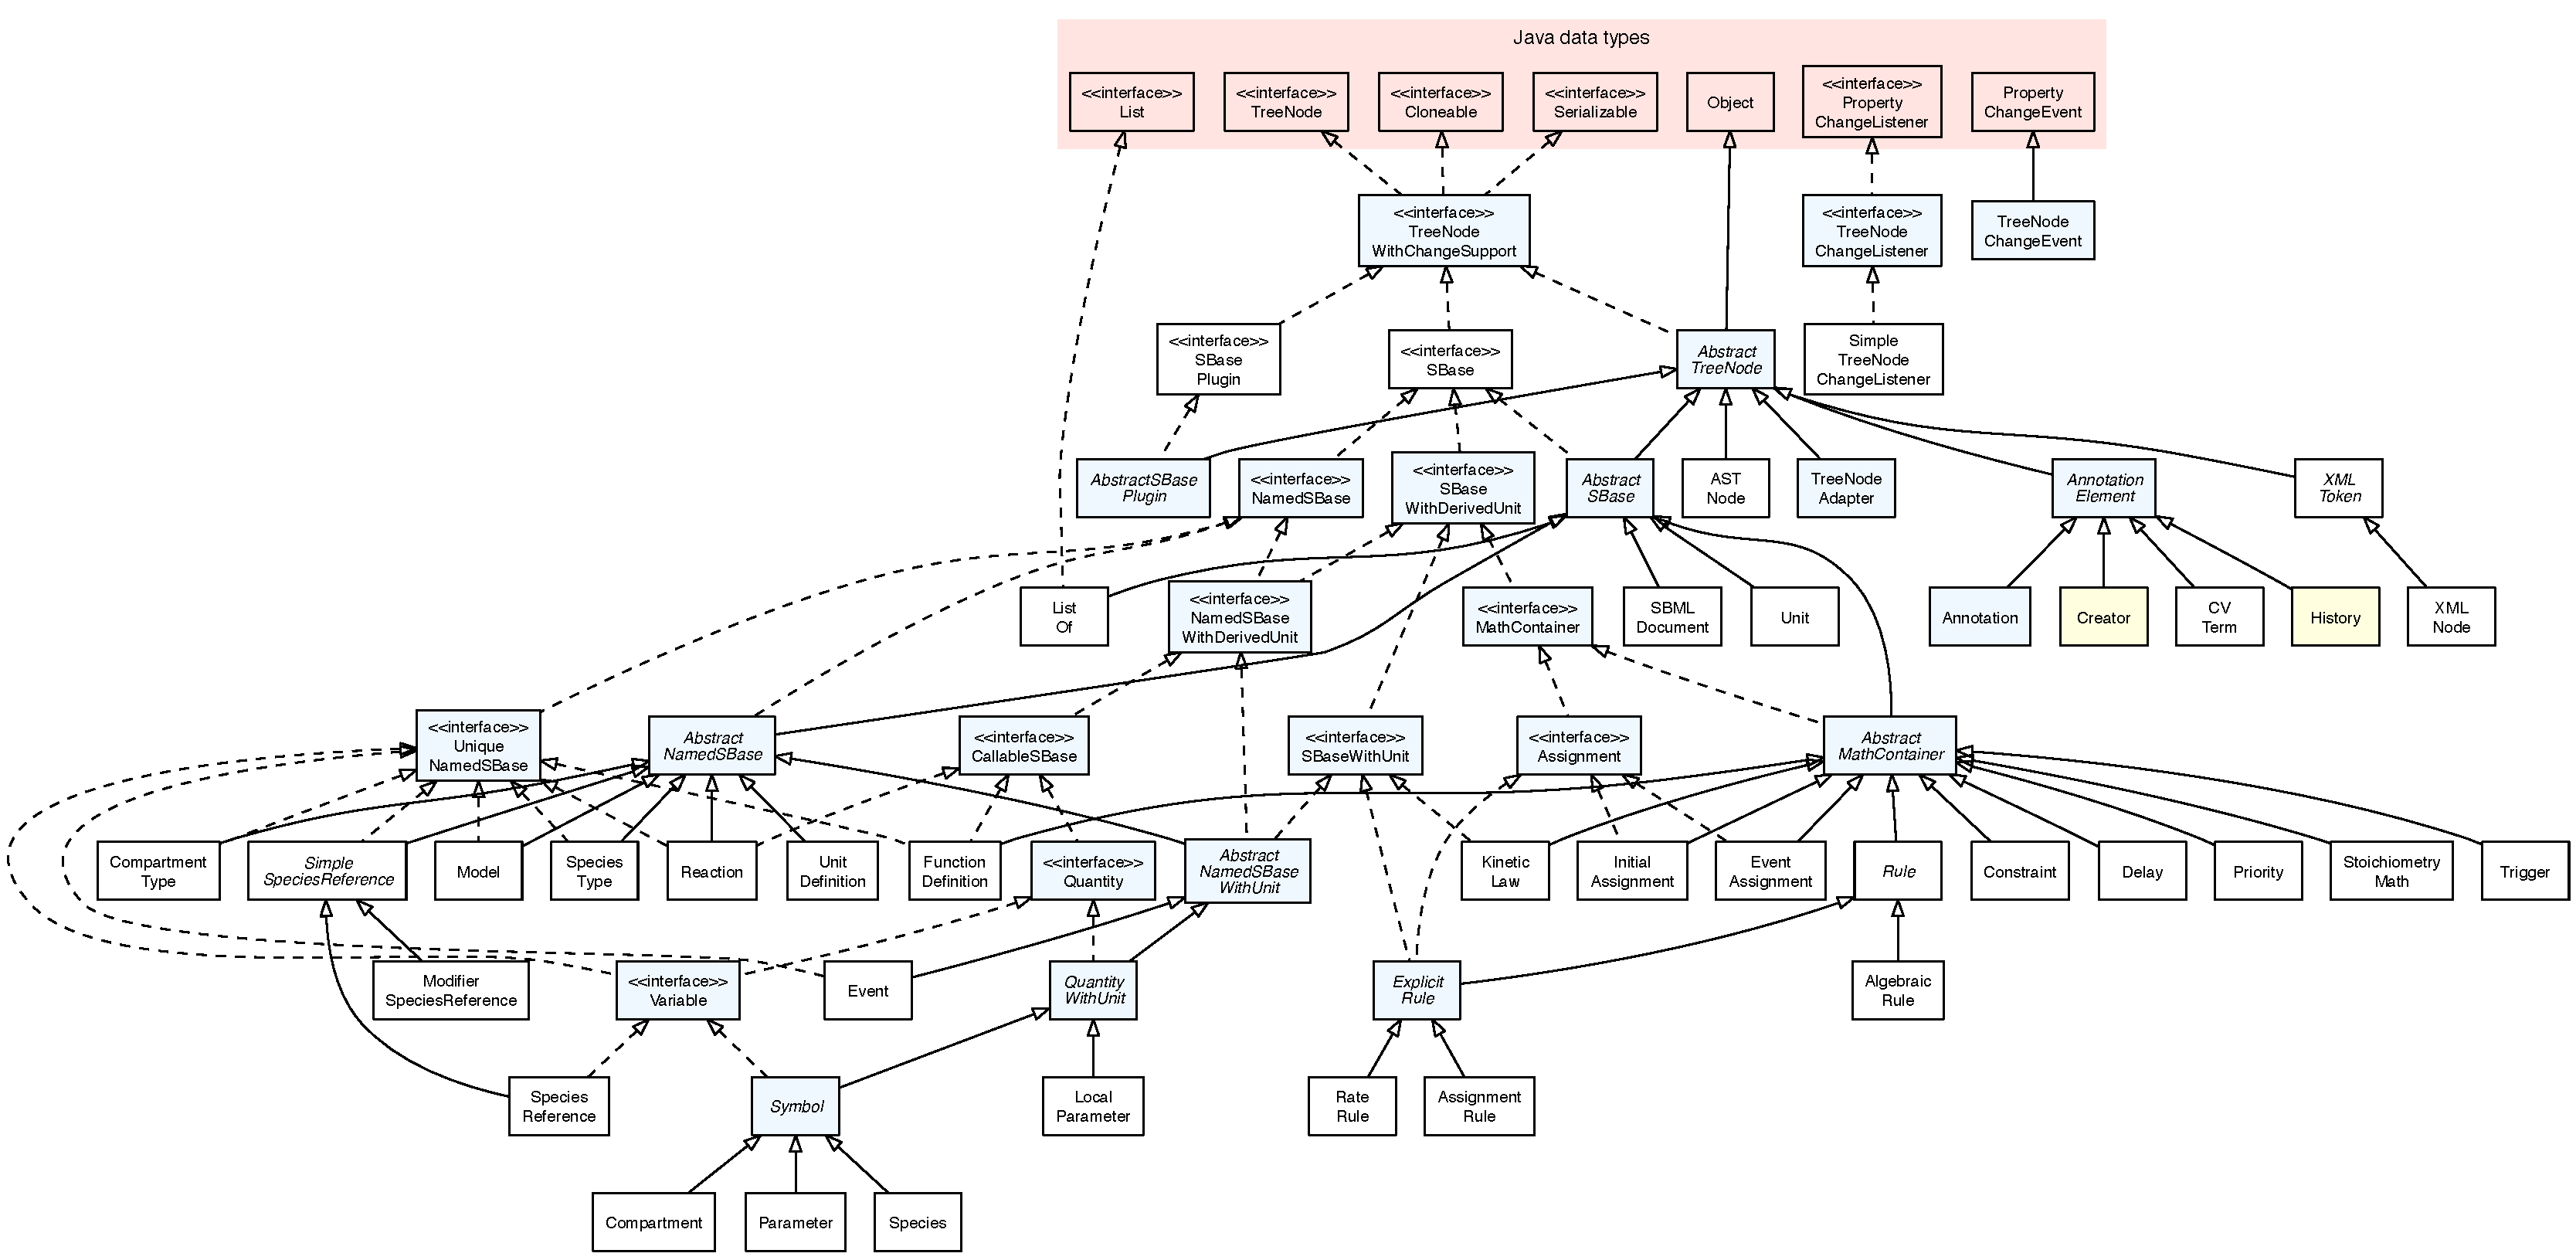
\includegraphics[width=0.97\textwidth]{../common/img/FullTypeHierarchy.pdf}
  \caption[The type hierarchy of the main SBML constructs in JSBML]{The
    type hierarchy of the main SBML constructs in JSBML. The elements
    colored in yellow, \code{Creator} and \code{History}, correspond to
    \code{ModelCreator} and \code{ModelHistory} in libSBML. Elements
    colored in blue are additional, in most cases abstract, data types in
    JSBML that do not have corresponding features in libSBML. Many other
    classes and interfaces in this diagram have no equivalent in libSBML,
    but offer more powerful capabilities for Java programmers. By making
    \SBase extend the interface \TreeNodeWithChangeSupport (another class
    defined by JSBML), which in turn extends the Java interfaces
    \code{Cloneable}, \code{Serializable}, and \TreeNode. All subclasses
    of \code{SBase} also provide the functionality of these classes and
    interfaces. In JSBML, even SBML components that are not defined by
    SBML as actually being derived from \code{SBase} are nevertheless
    derived from \TreeNodeWithChangeSupport; thus, they (and all their
    subclasses) share many common methods and attributes, which makes them
    easy to use when wherever instances of \TreeNode or operations across
    hierarchies of objects are needed. In order to support SBML Level~3
    packages, JSBML version 1.0 adds the interface \SBasePlugin and its
    abstract implementation \AbstractSBasePlugin (shown marked
    with a red border in this diagram).} 
  \label{fig:TypeHierarchy}
\end{sidewaysfigure}

Wherever multiple SBML elements defined in at least one SBML Level/Version
combination \index{SBML!specification} share attributes, JSBML
\index{JSBML!type hierarchy} provides a common superclass, or at least a
common interface, that gathers methods for manipulating the shared
properties. Consequently, JSBML's type hierarchy
\index{application programming interface!JSBML} is richer than libSBML's (see
\vrefrange{fig:TypeHierarchy}{fig:MathContainerHierarchy}).

Just as in libSBML, \index{application programming interface!libSBML} all
SBML objects derived from SBML's \SBase extend the JSBML abstract class
\SBase, but in JSBML, \SBase is an interface rather than an object class.
This allows more complex relations to be defined between derived data
types. In contrast to libSBML, JSBML's \SBase extends the interface
\TreeNodeWithChangeSupport, which in turn extends three other interfaces:
\Cloneable, \Serializable, and \TreeNode (\fig*{fig:SBase}).
This brings with it various advantages. One is that, because all elements
defined in JSBML \index{cloning} override the \code{clone()} method from
the class \code{java.lang.Object}, \index{Object@\code{Object}} all JSBML
elements can be deeply copied and are therefore \emph{cloneable}. Further,
extending the interface \Serializable makes it possible for JSBML
\index{application programming interface!JSBML} objects to be stored in
binary form without having to write them explicitly to an SBML file.
\index{SBML!XML file} In this way, programs can easily load and save their
in-memory objects or send data structures across a network connection
without the need of additional file encoding and subsequent parsing.

The third interface extended by \SBase, \TreeNode is defined in Java's
\emph{Swing} \index{graphical user interface!Swing} package; however,
\TreeNode is actually independent of any graphical information.  (We hasten
to add that JSBML does \emph{not} depend on any particular graphical user
interface, and no other classes are initialized when loading \TreeNode from
Java Swing.)  \TreeNode defines recursive methods on hierarchically
structured data types, such as iteration over all successors. This means
that, if a developer so desires, all instances of JSBML's \SBase interface
can be passed directly to the Java Swing \index{graphical user
  interface!Swing} class \JTree \index{graphical user
  interface!\code{JTree}} for easy visualization. The program shown in
\fig{fig:JSBMLvisualizer-source} (and whose output is presented in
\fig{fig:JSBMLvisualizer-output}) demonstrates the simple code
needed to parse an SBML file \index{SBML!XML file} and immediately display
its contents in a \JFrame. \index{graphical user interface!\code{JFrame}}
The \ASTNode class in JSBML is also derived from all these three interfaces
and can hence be cloned, serialized, and visualized in the same way.

\begin{figure}[hb]
 \centering
 \vspace*{2ex}
 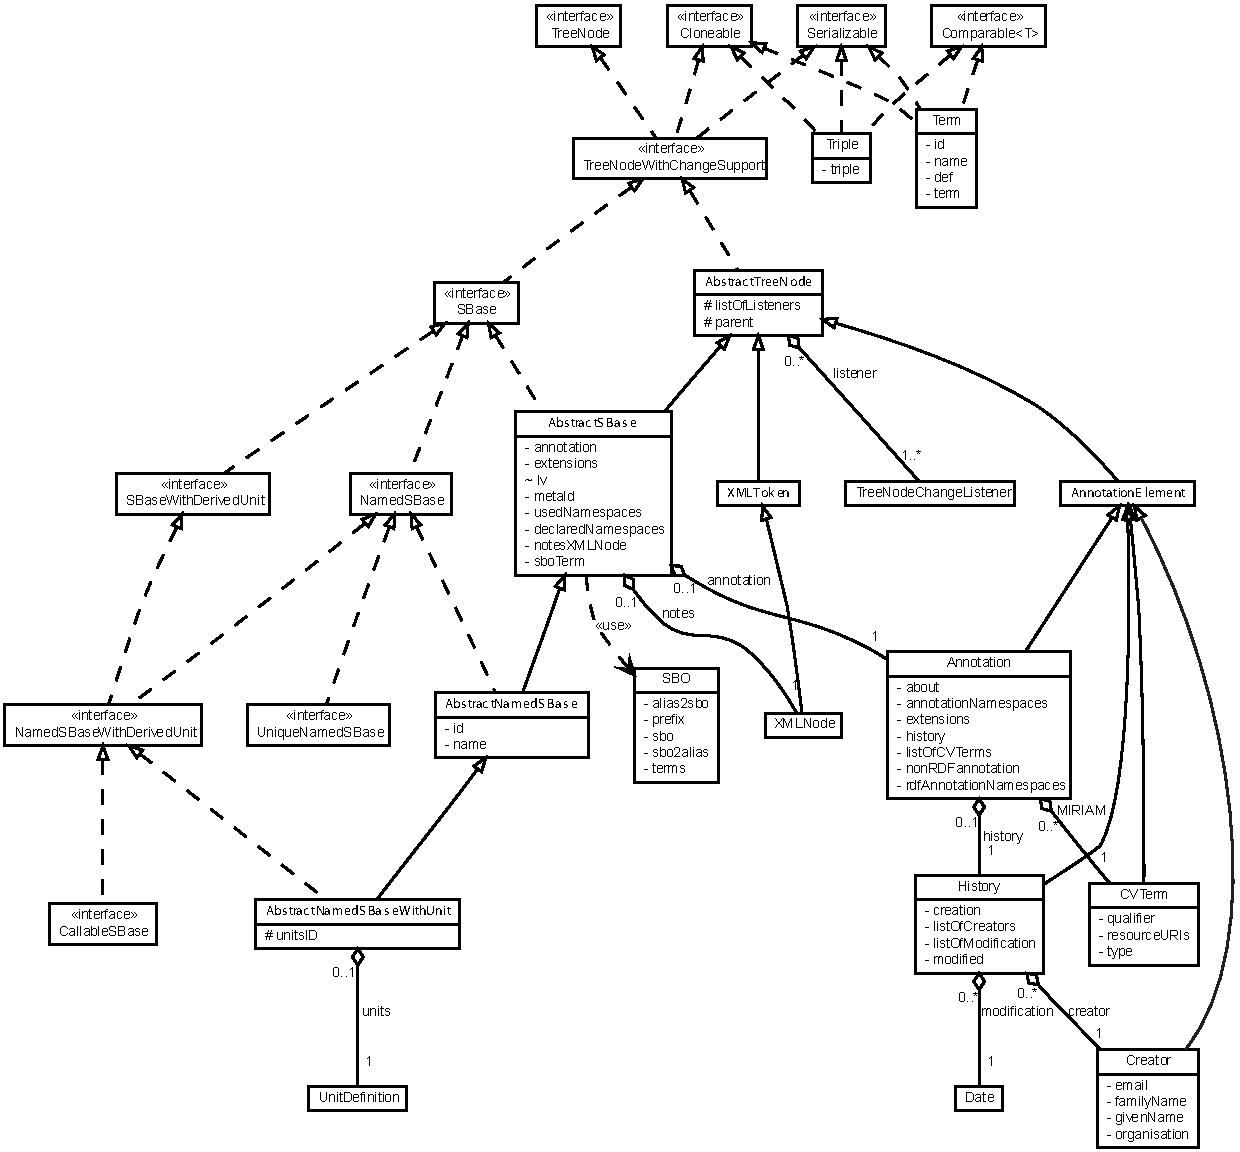
\includegraphics[width=\textwidth]{../common/img/SBase.pdf}
 % SBase.pdf: 1001x568 pixel, 72dpi, 35.31x20.04 cm, bb=0 0 1001 568
 \caption[The interface \code{SBase}]{The interface \SBase. This figure
   shows the most important top-level data structures in JSBML, with a
   focus on the differences compared to libSBML. For the sake of clarity,
   we have omitted all the methods on the classes shown here. As can be
   seen in this diagram, all data types that
   represent SBML constructs in JSBML extend \AbstractTreeNode.
   Derivatives of \SBase extend either one of the two abstract
   classes \AbstractSBase or \AbstractNamedSBase, which in turn
   also extend \AbstractTreeNode. The class \SBO implements
   facilities for parsing the ontology\index{Ontology} file provided on the
   SBO web site (\url{http://www.ebi.ac.uk/sbo/main/}) in OBO format (Open
   Biomedical Ontologies), using a parser provided by the BioJava
   project~\citep{Holland2008}. \SBO stores its ontology in
   the classes \code{Term} that are interrelated in \code{Triples}
   consisting of subject, predicate, and object (each being an instance of
   \code{Term}).}
 \label{fig:SBase}
\end{figure}


\subsection{Common interface for hierarchical structures: \codeNC{AbstractTreeNode}}%
\label{sec:AbstractTreeNode}
\index{TreeNode!AbstractTreeNode@\code{AbstractTreeNode}}

When reading the SBML specifications~\citep{Hucka2003, Hucka2008,
  Hucka2010a}, \index{SBML!specification} it quickly becomes apparent that
an SBML model has a tree-shaped, hierarchical structure, with \SBase being
the superclass of nearly all other SBML components. In JSBML, other kinds of
objects besides \SBase are also organized hierarchically within an
\SBMLDocument.  To unify the programming interfaces for all of these kinds
of objects, JSBML defines abstract data types as top-level ancestors for
its \SBase implementation as well as all other hierarchical elements, such
as \Annotation, \ASTNode, \Creator, \CVTerm, \History, and \XMLNode (for
notes in XHTML \index{XHTML} format).

As mentioned above, the interface \TreeNodeWithChangeSupport defines a
cloneable and serializable version of \TreeNode. (See the diagram in
\fig{fig:SBase}.) In addition, it also provides methods to notify
dedicated \TreeNodeChangeListener class objects about any changes within
the data structure. Its abstract implementation, \AbstractTreeNode,
implements many of the methods inherited from \TreeNodeWithChangeSupport
and also maintains a list of change listeners (implemented as
\TreeNodeChangeListener{}s). Furthermore, this class contains a basic
implementation of the methods \code{equals} and \code{hashCode}, which both
make use of a recursive call over all descendants within the hierarchical
SBML data structure. By basing the object definitions on this class, the
implementation of all derived classes has become much simpler.


\subsection{Common root of SBML components: \codeNC{AbstractSBase}}

With \SBase being an interface rather than an object class, most SBML-related
object classes in JSBML extend the abstract implementation \AbstractSBase, as
shown in \fig{fig:SBase}.  One of the features of this abstract class is
that it tracks the SBML Level and Version of every concrete object
implementing it.  The need for tracking each object's Level+Version
combination individually (a feature shared with libSBML) may seem odd at
first.  The need arises because a software system may need to work with more
than one combination at a given time; it may also need to create individual
SBML components before they are hooked into \SBMLDocument, which again
requires that individual objects know the SBML Level and Version for which
they were created.


\subsection{Interface for SBML components with identifiers: \codeNC{NamedSBase}}

Some classes of objects derived from \SBase in SBML contain an identifier,
colloquially often simply called the \emph{id}. JSBML gathers all elements
that have SBML identifiers under the common interface \NamedSBase. The JSBML
class \AbstractNamedSBase extends \AbstractSBase and implements this
interface.  

The interface \UniqueNamedSBase is shared by those elements whose
identifiers must be unique within the model. The identifiers of all instances
of \NamedSBase that do not implement \UniqueNamedSBase but belong to the same
group, such as all \UnitDefinition instances, must be unique if these identifiers are
defined. The Boolean method \code{isIdMandatory()} on \NamedSBase indicates
if an identifier must be defined for an element in order to create a valid
SBML data structure.  This is required in JSBML because the \Model object
stores direct pointers in the form of a hash from the identifier of the
corresponding object if \code{isIdMandatory()} returns \code{true}. 
The method decides if registering an element for its identifier has been a
success even if no identifier has been defined for this element. It is
necessary to have the method \code{isIdMandatory()}, because even if something
implements \UniqueNamedSBase, the identifier might be optional, as is the
case with \SimpleSpeciesReference. But the \Model class has to decide if and
where to store the identifier-to-element mapping in its hash. For details, see
the \Model class, where you can find some methods named \code{registerIds}, in
which the Boolean method is called.

The only elements with non-unique identifiers are \UnitDefinition, whose
identifiers exist in a separate namespace, and \LocalParameter, whose
identifiers may shadow the identifiers of global elements. (However, within a
given list of \UnitDefinition objects or list of \LocalParameter objects,
duplicate identifiers are not allowed.)

Internally, JSBML only uses the attribute \emph{id} for unique identifiers.
When you work with SBML Level~1, where the SBML specifications only define
name attributes (i.e., no identifiers) for elements, calls to
\code{setName(String)} are redirected to \code{setId(String)}. For all other
SBML Levels, an SBML element's \emph{name} can be specified separately from
the \emph{id} and does not have to be unique. In contrast to the identifier,
there is no syntax check on the name because it can consist of any UTF-8
character. The class that manipulates identifiers and names is
\AbstractNamedSBase; all classes with identifiers and names (optional
or mandatory) are derived from \AbstractNamedSBase. Accordingly,
\code{getName()} returns the identifier if working with SBML Level~1, but
internally it is redirected to \code{getId()}. For all other Levels,
\code{getName()} and \code{getId()} may yield different values, depending on
what is set for the class.

Summarizing, all classes in JSBML that implement the (empty) interface
\UniqueNamedSBase are types of \SBase, more precisely \NamedSBase (interface)
or \AbstractNamedSBase (abstract class), whose identifier must be unique through
the entire SBML model if it is set. \UnitDefinition and \LocalParameter do not
implement this interface. These are {\NamedSBase}s, whose identifier may
override the identifiers of elements that do implement \UniqueNamedSBase, but
not other {\UnitDefinition}s or other {\LocalParameter}s within the same
\KineticLaw. A Level and Version dependent syntax check ensures the validity of
identifiers. In this way, the correctness of the model is ensured and the \Model
class can centrally maintain hashes for elements with identifiers. This
significantly speeds up the getXXX(String id) methods.


\subsection{Interface for SBML components with units: \codeNC{SBaseWithDerivedUnit}}

Many SBML components represent some quantitative value with which a unit of
measurement is associated. However, the numerical value of an SBML
component does not necessarily have to be defined explicitly in the model;
it may instead be determined by a mathematical formula contained in a given
\SBase object in the model.  This implies that the unit associated with the
value may be derivable.  In JSBML, the interface \SBaseWithDerivedUnit is
used to represent all components that either explicitly or implicitly
contain some unit.  \fig{fig:Variable} shows this part of JSBML's
type hierarchy in more detail.

\begin{figure}[b]
  \vspace*{2ex}
  \centering
  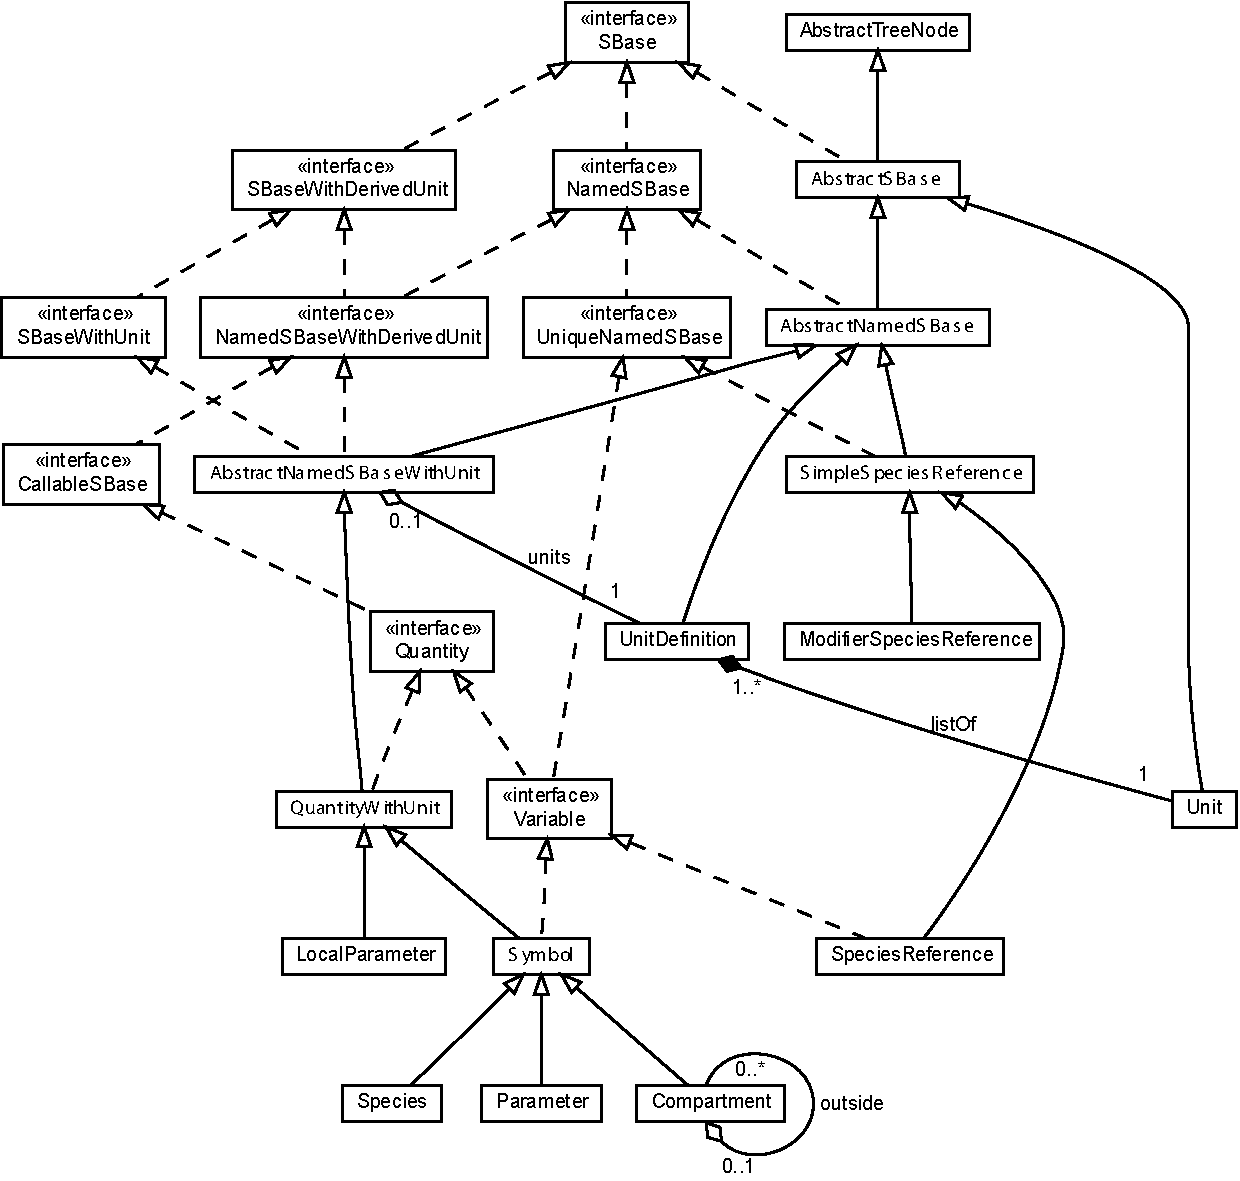
\includegraphics[width=\textwidth]{../common/img/Symbol.pdf}
  % Symbol.pdf: 596x587 pixel, 72dpi, 21.03x20.71 cm, bb=0 0 596 587
  \caption[The interface \Variable]{Part of JSBML's type
    hierarchy focusing on the interface \Variable.  In JSBML,
    those components of a model that may change their value during a
    simulation are referred to as \emph{variables}. The class \Symbol serves
    as the abstract superclass for variables that have units of measurement
    associated with them. Instances of \Parameter do not contain any
    additional fields. In \Species, a Boolean switch decides whether its
    value is to be interpreted as an initial amount or as an initial
    concentration. In contrast to \Variable{}s, \LocalParameter{}s represent
    constant unit-value pairs that can only be accessed within their
    declaring \KineticLaw. \index{SBML!variable}}
 \label{fig:Variable}
\end{figure}


If the SBML component can be addressed with an identifier (which means that
it has an \code{id} field in SBML), it will also implement the JSBML
interface \NamedSBaseWithDerivedUnit, and if it can appear within a formula
(which in JSBML, is represented using \ASTNode, discussed further below),
the entity will further implement the interface \CallableSBase, a special
case of \code{NamedSBaseWithDerivedUnit}.  When a component can be assigned
a unit explicitly, in JSBML the \SBaseWithUnit serves as its superclass.
JSBML further defines the convenience class \AbstractNamedSBaseWithUnit; it
extends \AbstractNamedSBase and implements interfaces \SBaseWithUnit
and \NamedSBaseWithDerivedUnit.  All elements derived from this abstract
class may therefore declare a unit and can be addressed using an
unambiguous SBML identifier.

In JSBML, the interface \Quantity describes an element that is associated
with a value, has at least a derived unit, and can be addressed using its
unambiguous identifier. JSBML uses the abstract class \QuantityWithUnit for
a \Quantity that explicitly declares its unit.  If the corresponding SBML
component includes a Boolean \index{Boolean} flag to indicate whether it is
a constant \index{SBML!constant} or a variable, JSBML
represents such a type using the interface \Variable.

SBML variables \index{SBML!variable} that have a defined unit are
represented as \Symbol objects.  (See \fig{fig:Variable}.) Thus,
the SBML elements \Compartment, \Parameter, and \Species are all special
cases of \Symbol in JSBML.  The specification of \SBMLthree introduced
another type of \Variable, which does not explicitly declare its unit:
\SpeciesReference.  Level~3 also introduced \LocalParameter, which is a
\QuantityWithUnit but not a \Variable because it is always constant.
\sec{sec:assignment-interface} explains the interfaces used for
changing the values of \Variable{}s.


\subsection{Interface for SBML components containing a mathematical
  formula: \codeNC{MathContainer}} 

The interface \MathContainer in JSBML gathers all those elements that may
contain mathematical expressions encoded in abstract syntax trees (i.e.,
instances of \ASTNode).  The abstract class \AbstractMathContainer serves
as actual superclass for the majority of the derived types.
\vrefrange{fig:MathContainer}{fig:MathContainerHierarchy} give a
better overview of how these data structures are organized and how they
relate to each other and other ones in JSBML.

\begin{figure}[hb]
 \centering
 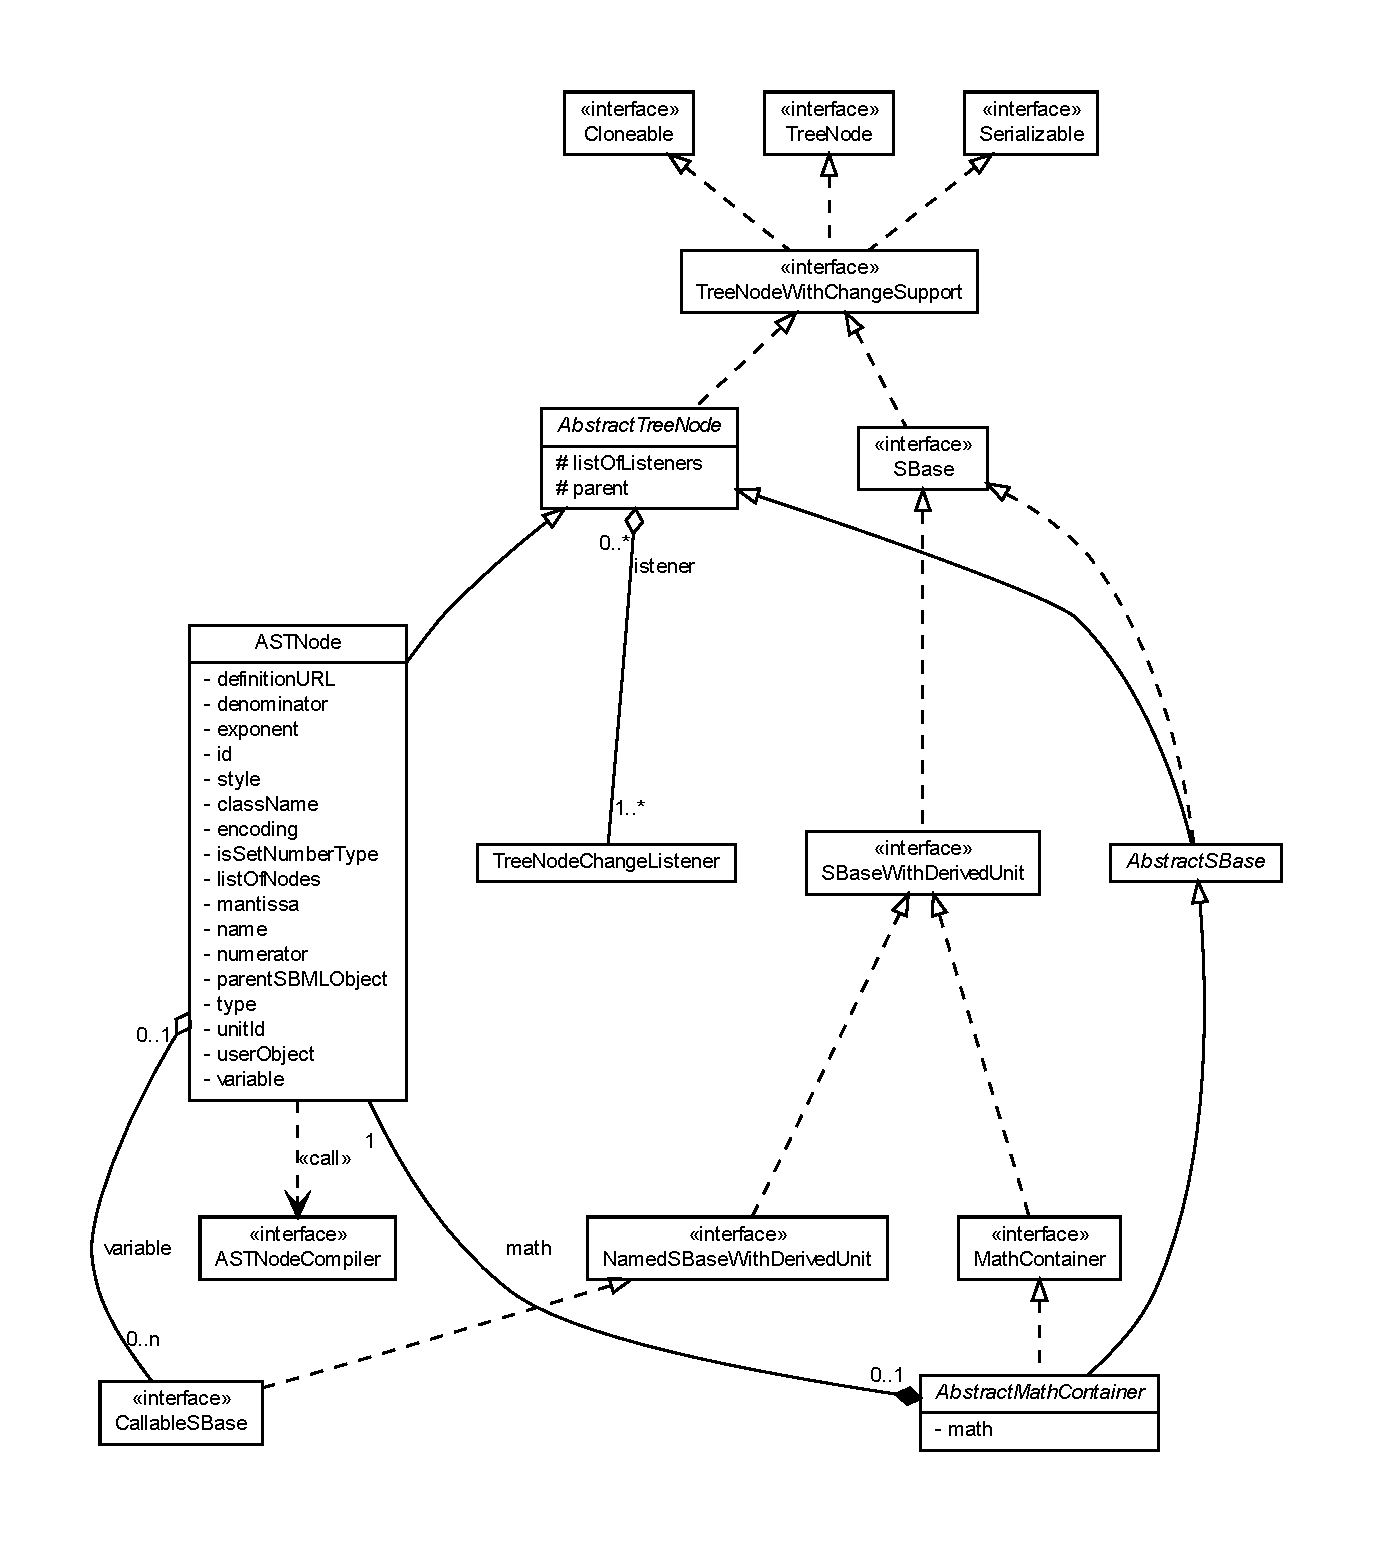
\includegraphics[width=\textwidth]{../common/img/ASTNode.pdf}
 % MathContainerClass.pdf: 557x396 pixel, 72dpi, 19.65x13.97 cm, bb=0 0 557 396
 \caption[Abstract syntax trees]{Abstract syntax trees (ASTs). The class
   \AbstractMathContainer serves as the superclass for several model
   components in JSBML. It provides methods to manipulate and access an
   instance of \ASTNode, which can be converted to or read from text
   strings containing formulas in a C-like infix syntax. Internally,
   \AbstractMathContainer{}s only deal with instances of \ASTNode. It
   should be noted that these abstract syntax trees do not implement the
   \SBase interface, but extend \AbstractTreeNode instead.}
 \label{fig:MathContainer}
\end{figure}

\begin{sidewaysfigure}
 \centering
 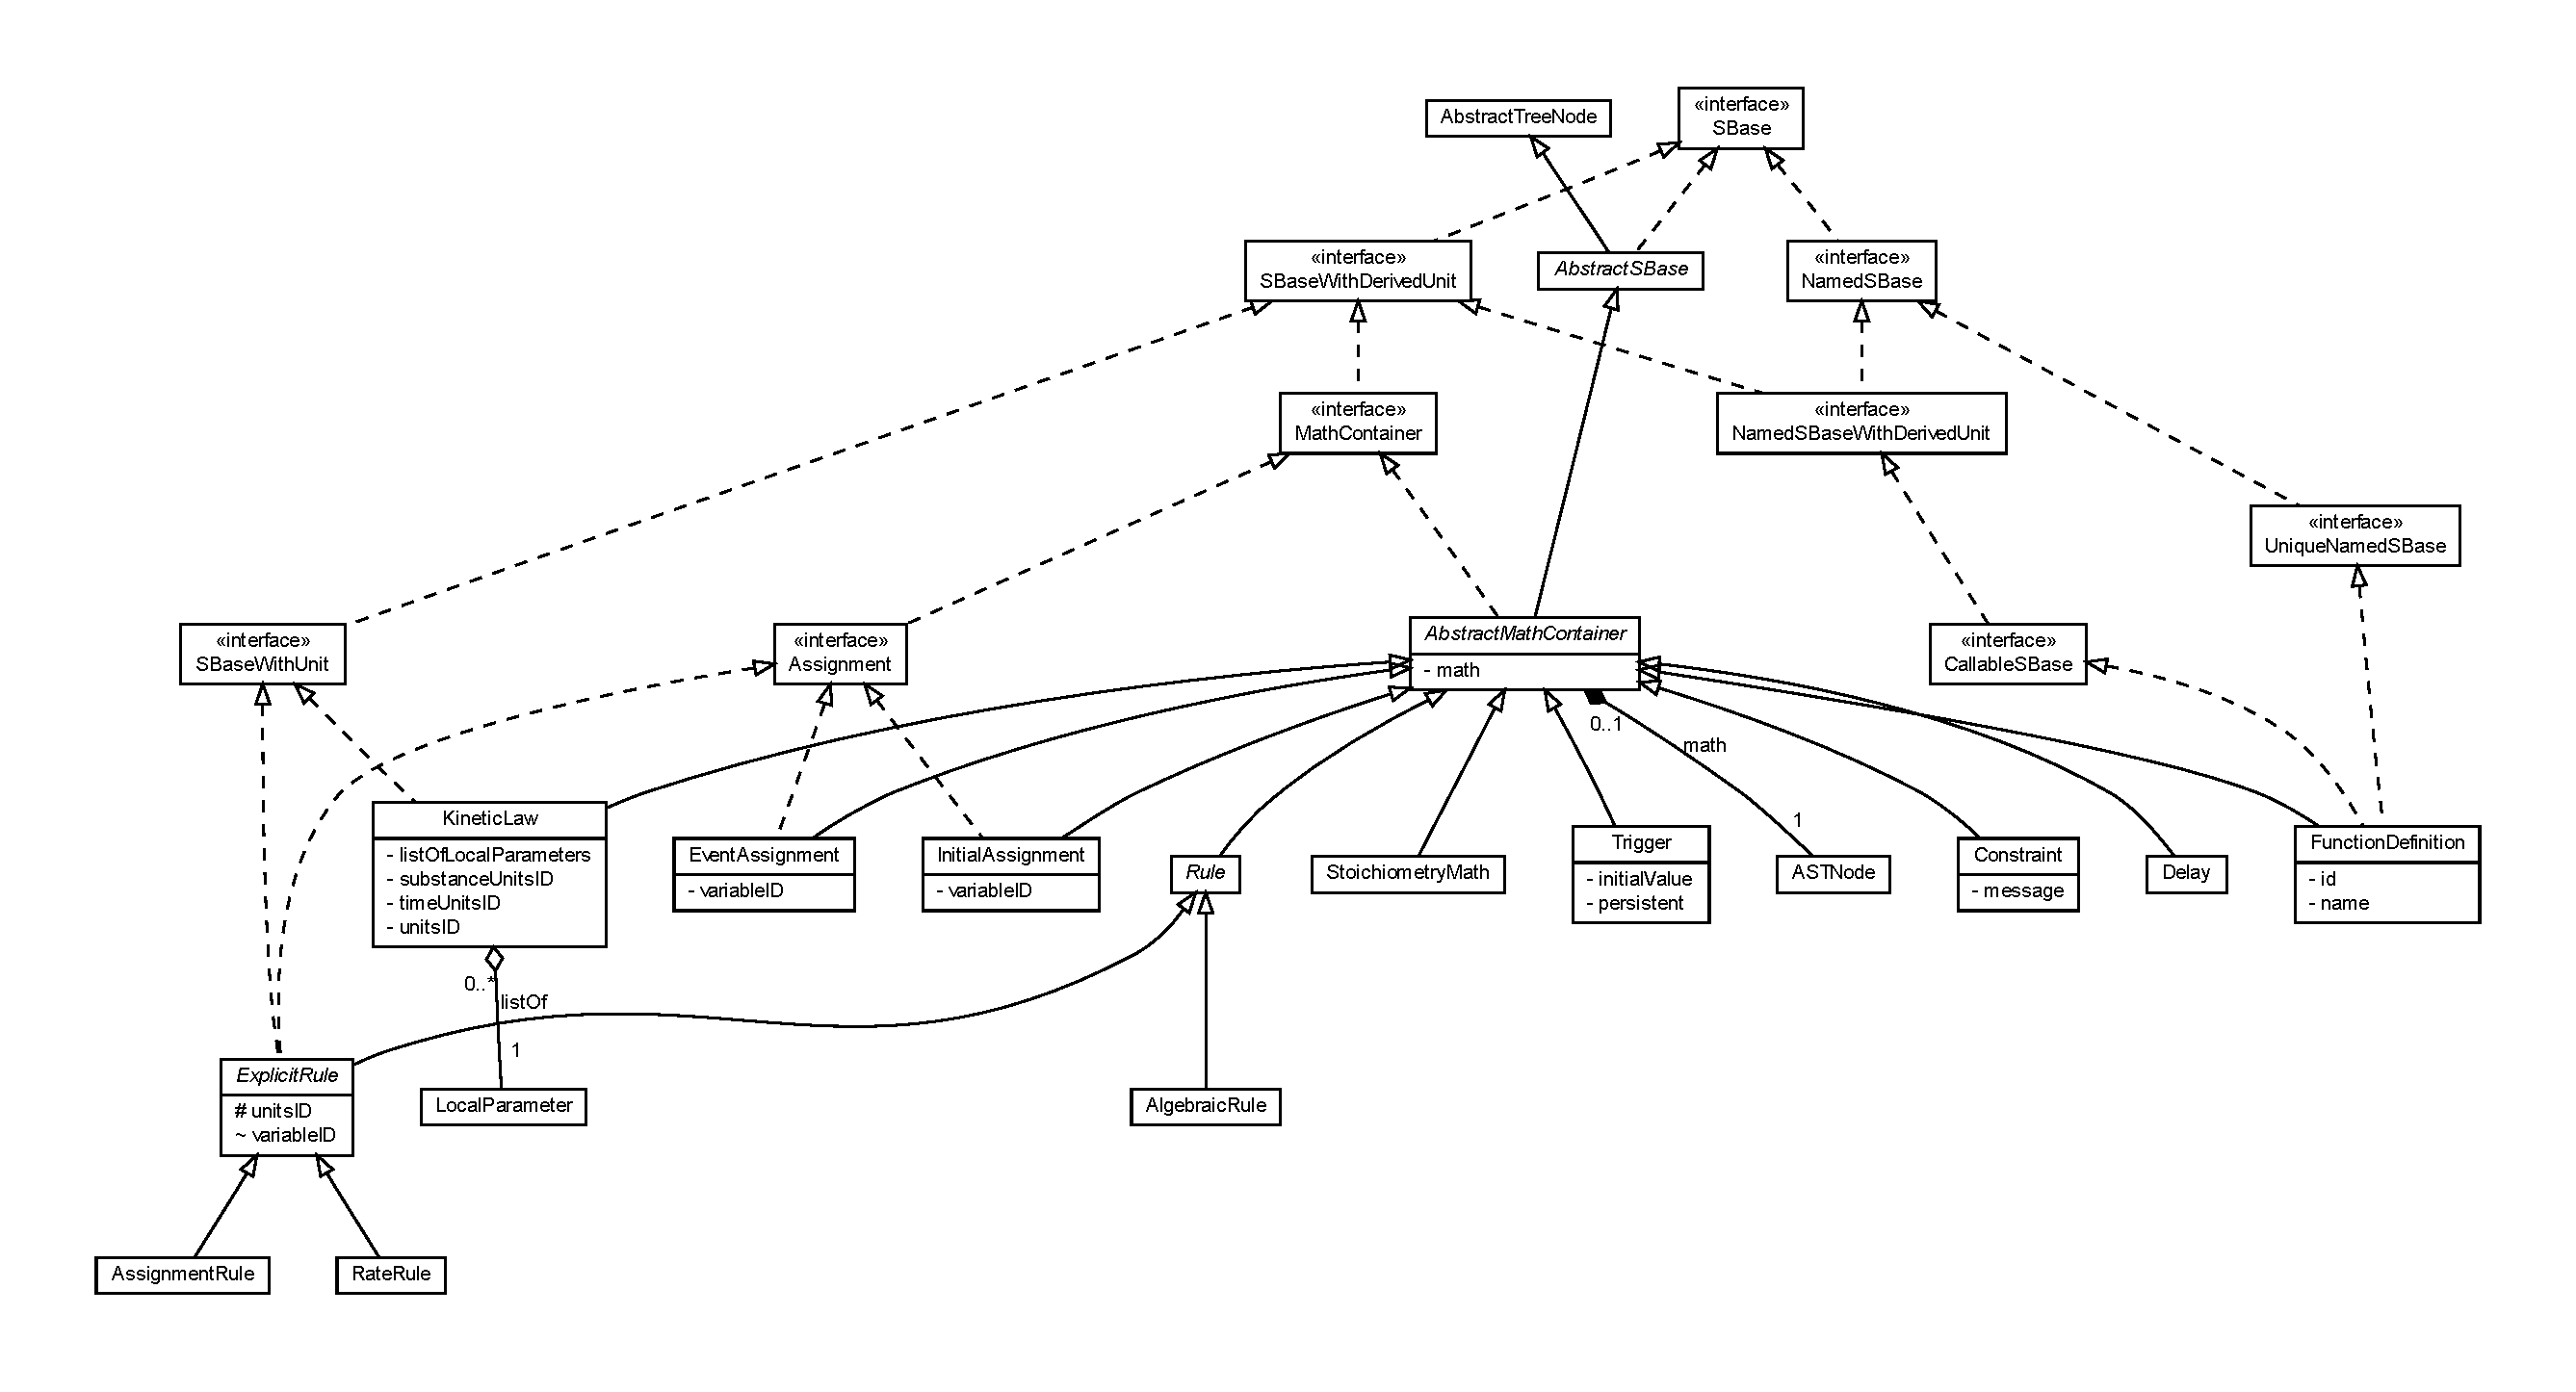
\includegraphics[width=\textwidth]{../common/img/MathContainer.pdf}
 % MathContainerClass.pdf: 557x396 pixel, 72dpi, 19.65x13.97 cm, bb=0 0 557 396
 \caption[Containers for mathematical expressions]{Containers for
   mathematical expressions. The interface \MathContainer, particularly its
   directly derived class \AbstractMathContainer, constitutes the
   superclass for all elements that store and manipulate mathematical
   formulas in JSBML.  The formulas themselves are stored in the form of
   \ASTNode objects. These can be evaluated using an implementation of
   \ASTNodeCompiler. Note that some classes that extend
   \AbstractMathContainer do not contain any of their own additional fields
   or methods.  This is the case for \Delay, \Priority, \StoichiometryMath,
   and \AlgebraicRule.}
 \label{fig:MathContainerHierarchy}
\end{sidewaysfigure}


\subsection{Interface for SBML components that may change the value of
  a variable: \codeNC{Assignment}}
\label{sec:assignment-interface}
\index{JSBML!assignment@\code{Assignment}}

JSBML provides a unified interface, \Assignment, for all objects that may
change the value of some variable in SBML. \index{SBML} This interface uses
the term \emph{variable} for the element whose value can be changed
depending on some mathematical expression that is also present in the
\Assignment (because the interface \Assignment extends the interface
\MathContainer).  Therefore, an \code{Assignment} contains methods such as
\code{set}-/\code{getVariable(Variable v)} and also \code{isSetVariable()}
as well as \code{unsetVariable()}.

In addition, JSBML also provides the methods
\code{set}-/\code{getSymbol(String symbol)} in the \InitialAssignment class
to make it easier to switch from libSBML to JSBML.  However, in JSBML, the
preferred way \index{JSBML!variable@\code{Variable}} is to apply the
methods \code{setVariable()}, either with \String or \Variable instances as
arguments.  \fig{fig:MathContainerHierarchy} shows the class
hierarchy surrounding the \Assignment interface in more detail.


\section{Differences between the APIs of JSBML and libSBML}
\label{sec:api-differences}

We strove to make JSBML be closely compatible with libSBML. However,
because of the different programming languages used,
some differences are impossible to overcome.
In other cases, an exact translation from libSBML's C/C++ \index{C}
code to Java would be inelegant and unnatural for Java users,
conflicting with another important goal of JSBML: to provide
an API \index{application programming interface!Java} whose classes and
methods behave, and are organized like, those in other Java libraries.

In this section, we discuss the most important differences in the APIs of
JSBML \index{application programming interface!JSBML} and libSBML.
\index{application programming interface!libSBML} We also provide some
examples of how the classes and methods in JSBML may be used.


\subsection{Level and Version \codeNC{ValuePair}}

In libSBML, the Level and Version information is recorded as individual
integers; by contrast, in JSBML it is stored in a generic object, \ValuePair,
stored within an \AbstractSBase instance. The class \ValuePair implements the
Java interface \Comparable and takes two values of any type that both also
implement \Comparable.  Storing the information in this way allows users to
check for a specific Level/Version combination more naturally, as the example
in \fig{fig:LevelVersionCheck} demonstrates. The method
\code{getLevelAndVersion()} in \AbstractSBase delivers an instance of
\ValuePair with the Level and Version combination for the respective element.

\begin{figure}[bh]%
  \begin{example}
if (mySBase.getLevelAndVersion().compareTo(Integer.valueOf(2), Integer.valueOf(2)) < 0) {
  throw new IllegalArgumentException("Cannot create a " + mySBase.getElementName() + 
  		" with Level = " + getLevel() + " and Version = " + getVersion() + ".");
}\end{example}
  \caption{Example program fragment showing how to check for a minimal
    expected SBML Level/Version combination.}
  \label{fig:LevelVersionCheck}
\end{figure}


\subsection{Abstract syntax trees for mathematical formulas}

Both libSBML and JSBML define a class called \ASTNode for in-memory storage
and evaluation of abstract syntax trees (ASTs) that represent mathematical
formulas. These can be parsed either from \String{}s containing formulas in a
C-like infix syntax, or from a MathML \index{MathML} representation.  JSBML's
\ASTNode class provides various methods to transform ASTs to other formats,
for instance, \code{String}s in \LaTeX \index{LaTeX@\LaTeX} syntax.  Several static methods also
make it easy to create syntax trees.  The next example creates a new
\ASTNode which represents the sum of the two other nodes:

\begin{example}
ASTNode myNode = ASTNode.sum(myLeftAstNode, myRightASTNode);
\end{example}

SBML specifies that mathematical formulas may contain references to the
following kinds of components in a model: \Parameter{}s,
\LocalParameter{}s, \FunctionDefinition{}s, \Reaction{}s, \Compartment{}s,
\Species, and in \SBMLthree, \SpeciesReference{}s.  In JSBML, all of these
classes implement a common interface, \CallableSBase, which extends
the interface \NamedSBaseWithDerivedUnit. This organization ensures that
only identifiers of these particular SBML components can be set in
instances of \ASTNode.


\subsubsection{Constructors and other methods for \CallableSBase}

JSBML provides useful constructors and methods to work with instances of
\CallableSBase.  The \code{set} method changes the type of an \ASTNode to
\ASTTypeName and directly sets the name to the identifier of the given
\CallableSBase.  The \code{get} method looks for the corresponding object in
the \Model and returns it. If no such object can be found or the type of the
\ASTNode is something different from \ASTTypeName, it throws an exception.

\begin{example}[title={Getter and setter for \CallableSBase.}]
public void setVariable(CallableSBase variable) { ... }

public CallableSBase getVariable() { ... }
\end{example}

The following are examples of methods for creating and manipulating complex
ASTs.  JSBML provides several static methods (such as \code{sum} shown above)
that create small trees from objects in memory.  Other methods, such as
\code{plus}, \code{frac} and \code{pow}, change existing tree structures:

\begin{example}[title={Some examples for convenience methods, some of
    them static methods, provided by JSBML for working with \ASTNode{}s.}]
public ASTNode plus(CallableSBase nsb) { ... }

public static ASTNode frac(MathContainer container,
      CallableSBase numerator, CallableSBase denominator) { ... }

public static ASTNode pow(MathContainer container,
      CallableSBase basis, CallableSBase exponent) { ... }
\end{example}

In contrast to the static \code{ASTNode.sum} function at the beginning of
this section, the \code{frac} and the \code{pow} methods above take instances
of \CallableSBase as their arguments instead of \ASTNode objects. Consequently, the
parent \MathContainer must be passed to the methods in order to ensure that
valid data structures are created. (In case of methods that take \ASTNode
objects as arguments, such as the static \code{ASTNode.sum}, the parent
\MathContainer can be taken from the first given node object.)

Finally, with the following \ASTNode constructors, dedicated single nodes can
be created whose type (from the enumeration \ASTType) will be \code{NAME} and
whose name will be set to the identifier of the given \CallableSBase.

\begin{example}
public ASTNode(CallableSBase nsb) { ... }

public ASTNode(CallableSBase nsb, MathContainer parent) { ... }
\end{example}


\subsubsection{The \codeNC{ASTNodeCompiler} class}

JSBML provides the interface \ASTNodeCompiler; it allows users to create
customized interpreters for the contents of mathematical formulas encoded
in abstract syntax trees. It is directly and recursively called from the
\ASTNode class and returns an \ASTNodeValue object, which wraps the
possible evaluation results of the interpretation.  As alluded to above,
JSBML provides several implementations of this interface; for instance,
\ASTNode objects can be directly translated to C language-like \String{}s,
\LaTeX, \index{LaTeX@\LaTeX} or MathML \index{MathML} for further
processing.  In addition, the class \UnitsCompiler, which JSBML uses to
derive the unit of an abstract syntax tree, also implements this interface.


\subsection{Compartments}

In \SBMLthree~\citep{Hucka2010a}, the domain of the attribute
\code{spatialDimensions} on \Compartment is no longer $\lbrace 0, 1, 2,
3\rbrace$, which can be represented with a \code{short} value in Java, and is
instead a real-numbered value (i.e., a value in $\mathbb{R}$), which requires
a \code{double} value in Java. For this reason, the method
\code{getSpatialDimensions()} in JSBML always returns a \code{double}
value. For consistency with libSBML, the \Compartment class in JSBML also
provides the redundant method \code{getSpatialDimensionsAsDouble()} that
returns the identical value; it is marked as a deprecated method.
\index{compartment!\code{getSpatialDimensions()}}%
\index{compartment!\code{getSpatialDimensionsAsDouble()}}%


\subsection{Model history}

Before \SBML Level~3, only the \Model object could have an associated
history, that is, a description about the person(s) who build the model,
including names, email addresses, modification and creation dates.  In
Level~3 of SBML, it is possible to annotate every construct with a
history. This is reflected in JSBML by the name of the corresponding
object---\History---whereas it is named \ModelHistory in libSBML.  All
instances of \SBase in JSBML contain methods to access and manipulate its
\History. Also, JSBML does not have libSBML's classes \ModelCreator
and \ModelCreatorList because JSBML gathers its \Creator objects in a generic
\code{List<Creator>} in the \History.


\subsection{Units and unit definitions}
\label{sec:units}

There are differences between libSBML and JSBML's interfaces for handling
units.  We describe them next.


\subsubsection{The exponent attribute of units}

In \SBMLthree~\citep{Hucka2010a}, the data type of the exponent attribute
of a \Unit object changed from \code{int} in previous Levels to
\code{double} values. To provide a uniform interface no matter which Level
of SBML is being dealt with, JSBML's method \code{getExponent()} only
returns \code{double} values. In libSBML, \code{getExponent()} always
returns \code{int}, and there is an additional method,
\code{getExponentAsDouble()}, to handle the cases with \code{double}
values.  JSBML provides \code{getExponentAsDouble()} for compatibility with
libSBML, but it is a redundant method in JSBML's case and therefore is marked
as deprecated.
\index{unit!getExponent()@\code{getExponent()}}%
\index{unit!getExponentAsDouble()@\code{getExponentAsDouble()}}%


\subsubsection{Predefined unit definitions}

A model in JSBML \index{unit!predefined units} always contains all
predefined units defined by SBML.  These can be accessed from an instance
of \code{Model} by calling the method \code{getPredefinedUnit(String
  unit)}.

MIRIAM annotations\index{annotations!MIRIAM} \citep{Novere2005} have been
an integral part of SBML models since Level~2 Version~2\index{SBML!Level~2
  Version~2}. Recently, the \index{Ontology} Unit Ontology
(UO)~\citep{unitontology} \index{annotations!unit ontology} has been
included in the set of supported ontology and online resources of MIRIAM
annotations~\citep{Novere2005}. Since all the predefined units in SBML have
corresponding entries in the UO, JSBML \index{unit!MIRIAM annotation}%
automatically equips those predefined units with the correct MIRIAM URI in
form of a controlled vocabulary term (\code{CVTerm}) if the SBML
Level/Version combination of the model supports MIRIAM annotations.  In
addition, the \code{enum} \code{Unit.Kind}
\index{unit!Unit.Kind@\code{Unit.Kind}}%
also provides methods to directly obtain the entry from the UO that
corresponds to a certain unit kind and also contains methods to generate
MIRIAM URIs accordingly. In this way, JSBML facilitates the annotation of
user-defined units and unit definitions with MIRIAM-compliant
\index{annotations!MIRIAM} information.


\subsubsection{Access to the units of an element}

In JSBML, all SBML components whose value can be associated with a unit of
measurement implement the interface \SBaseWithUnit.  This interface provides
methods to access an object representing the unit. Currently, the interface
is implemented by \AbstractNamedSBaseWithUnit, \ExplicitRule, and
\KineticLaw.  \fig{fig:TypeHierarchy} provides an overview about the
relationships between these and other classes and interfaces.

% FIXME

\AbstractNamedSBaseWithUnit is the abstract superclass for \Event and
\QuantityWithUnit.  In the class \Event, all methods to deal with units are
deprecated because the \code{timeUnits} attribute was removed in SBML
Level~2 Version~2\index{SBML!Level~2}. The same holds true for instances of
\ExplicitRule and \KineticLaw which both can only be explicitly populated
with units in SBML Level~1\index{SBML!Level~1} for \ExplicitRule and before
SBML in Level~2, Version~3\index{SBML!Level~2} for \KineticLaw. By
contrast, the abstract class \QuantityWithUnit serves as the superclass for
\LocalParameter and \Symbol, which is then the superclass of \Compartment,
\Species, and (global) \Parameter.  With \SBaseWithUnit being a subclass of
\SBaseWithDerivedUnit, users can access the units of such an element in two
different ways:

\begin{description}[font=\normalfont]

\item[\code{getUnit()}:] This method returns a \String representation of
  the unit kind or the identifier of a unit definition in the model \index{model} that has
  been directly set by the user during the life time of the element. If
  nothing has been declared, this method returns an empty \String.

\item[\code{getDerivedUnit()}:] This method gives either the same
  result as \index{unit!derived unit} \code{getUnit()} if some unit has
  been declared explicitly, or it returns the predefined unit of the
  element for the given SBML Level/Version combination.  If neither a
  user-defined nor a predefined unit is available, this method returns an
  \index{String@\code{String}!empty} empty \String.

\end{description}

% FIXME

For convenience, JSBML also provides corresponding methods to the ones
above for directly obtaining an instance of \UnitDefinition.  However, care
must be taken when obtaining an instance of \UnitDefinition from one of the
classes implementing \SBaseWithUnit because it might happen that the
model\index{model} containing this \SBaseWithUnit does actually not contain
the required instance of \UnitDefinition and the method returns a
\code{UnitDefinition} that has just been created for convenience from the
information provided by the class. It might therefore be useful for callers
to either check if the \Model{} contains this \UnitDefinition or to add it
to the \Model.

In case of \KineticLaw it is even more difficult, because SBML
Level~1\index{SBML!Level~1} provides the ability to set the substance unit
and the time unit separately. To unify the API
\index{application programming interface!JSBML}, we decided to also provide methods that
allow the user to simply pass one \UnitDefinition or its identifier to
\KineticLaw.  These methods then try to guess if a substance unit or time
unit is given. Furthermore, it is possible to pass a \UnitDefinition
representing a variant of substance per time directly. In this case, the
\KineticLaw will memorize a direct link to this \UnitDefinition in the
model\index{model} and also try to save separate links to the time unit and
the substance unit. However, this may cause a problem if the containing
\Model does not contain separate \UnitDefinition{}s for both entries.


\subsection{Cloning when adding child nodes to instances of \codeNC{SBase}}

When adding elements such as a \Species to a \Model, libSBML \index{cloning}
will clone the object and add the clone to the \Model. In contrast, JSBML
does not automatically perform cloning. This has the advantage that
modifications on the object belonging to the original pointer will also
propagate to the element added to the \Model; furthermore, this is more
efficient at run-time and also more intuitive for Java programmers. If
cloning is necessary, users should call the \code{clone()} method
explicitly. Since all instances of \SBase, and also \Annotation, \ASTNode,
\CVTerm, and \History, extend \AbstractTreeNode (which in turn implements the
interface \Cloneable---see \fig{fig:TypeHierarchy}), all these elements can
be cloned naturally.  However, when cloning an object in JSBML
\index{cloning}, such as an \AbstractNamedSBase, all children of this element
will recursively be cloned before adding them to the new element. This is
necessary because the data structures specified in SBML
\index{SBML!hierarchical structure} define a tree, in which each element has
exactly one parent. It is important to note that some properties of the
elements must not be copied when cloning:

\begin{enumerate}

\item The pointer to the parent node of the top level element that is
  recursively cloned is not copied and is left as \code{null}, because the
  cloned object will get a parent set as soon as it is added or linked again
  to an existing tree. Note that only the top-level element of the cloned
  subtree will have a \code{null} value as its parent. All subelements will
  point to their correct parent element.

\item The list of \TreeNodeChangeListener objects is used in all other
  \code{setXX()} methods. Copying pointers to these may lead to
  unexpected behaviors, because during deep cloning, the listeners of
  the old object will suddenly be informed about all changes to values within
  the new object.  In cloning, all values of all child elements
  will be touched, i.e., all listeners will have to be informed many times, but
  each time they will receive the same value. Since they do not
  extend the \Cloneable interface, we cannot clone them either; for this reason, the cloned
  object has no \TreeNodeChangeListener object attached to it. The user is responsible
  for adding \TreeNodeChangeListener{}s on the cloned object if they want to be
  notified of any changes to it.

\item Since release 1.0, JSBML supports storing user objects in any object
  derived from \AbstractTreeNode.  These user objects are organized in a map
  data structure with object as key type, pointing to arbitrary user-defined
  objects. Note that generally no deep cloning of these user objects is
  possible, but JSBML keeps a pointer to these user objects in the cloned
  element.

\end{enumerate}


\subsection{Exceptions}
\label{sec:exceptions}

In case of an error, JSBML \index{exception} methods will usually throw an
exception, whereas libSBML \index{exception!error codes} methods return a
numeric error code instead. The libSBML approach is rooted in the need to
support C-like languages, while exception handling is more natural in Java.
The JSBML approach of using exceptions helps programmers and users to avoid
creating invalid SBML data structures already when dealing with these in
memory. 

As per usual Java practice, JSBML methods declare that these may
potentially throw exceptions. In this way, programmers can be aware of
potential sources of problems already at the time of writing the source
code. Examples of the kinds of exceptions that JSBML methods may throw
include \ParseException, \index{exception!\code{ParseException}} which may
be thrown if a given formula cannot be parsed properly into an \ASTNode
data structure, and \InvalidArgumentException,
\index{exception!\code{InvalidArgumentException}} which may be thrown if
inappropriate values are passed to methods.

The following are some examples of situations that lead to exceptions:

\begin{itemize}

\item An object representing a constant\index{constant} such as a
  \Parameter whose \code{constant} attribute has been set to \code{true}
  cannot be used as the \Variable element in an \Assignment.
  \index{JSBML!assignment@\code{Assignment}}%
  \index{JSBML!variable@\code{Variable}}%
  \index{parameter!\code{Parameter}}%
  \index{parameter!\code{constant}}%

\item An instance of \Priority can only be assigned to an \Event{}s if its
  \code{level}\index{SBML!Level~3} attribute has at least been set to
  three.

\item Another example is the \InvalidArgumentException that is thrown when
  trying to set an invalid identifier \String for an instance of
  \AbstractNamedSBase.

\item JSBML keeps track of all identifiers within a model. For each
  namespace it contains a separate map of identifiers within the \Model. It
  is therefore not possible to assign duplicate identifiers in case of
  elements that implement the interface \UniqueNamedSBase.  For
  \UnitDefinition{}s and \LocalParameter{}s separate maps are
  maintained. Since local parameters are only visible within the
  \KineticLaw that contain these, JSBML will only prohibit having more
  than one local parameter within the same list that has the identical
  identifier. All these maps are updated upon any changes within the
  model. When adding an element with an already existing identifier for its
  namespace, or changing some identifier to a value that is already defined
  within this namespace, JSBML will throw an exception.

\item ``Meta'' identifiers must be unique through the entire SBML file. To
  ensure that no duplicate meta identifiers are created, JSBML keeps a map
  of all meta identifiers on the level of the \SBMLDocument, which is
  updated upon any change of elements within the data structure. In this
  way, it is not possible to map the meta identifier of some element to an
  already existing value or to add nodes to the SBML tree that contain a
  meta identifier defined somewhere else within the tree. In both cases,
  JSBML will throw an exception. Since meta identifiers can be generated in
  a fully automatic way (method \code{nextMetaId()} on
  \code{SBMLDocument}), users of JSBML should not care about these
  identifiers at all. JSBML will automatically create meta identifiers
  where missing upon writing an SBML file.  (See \sec{sec:find-methods}.)

\item In case that spatial dimension units of a \Species{} are defined
  whose surrounding \Compartment{} has zero dimensions or that has only
  substance units, JSBML also throws an exception.

\end{itemize}

Hence, you have to be aware of potential exceptions and errors when using
JSBML, \index{exception} on the other hand this will prevent you from doing
obvious mistakes. The class \SBMLReader in JSBML catches those errors and
exceptions. With the help of the logging utility, JSBML notifies users
about syntactical problems in SBML files. JSBML follows the rule that
illegal or invalid properties are not set.


\subsection{No interface  \codeNC{libSBMLConstants}}

JSBML does not contain an equivalent to libSBML's
\code{libSBMLConstants}. The reason is that in JSBML, constants are encoded
in a more natural Java fashion, \index{constant!\code{enum}}%
using the Java construct \code{enum}. For instance, all the fields starting
with the prefix \ASTTypePrefix{} have a corresponding field in the \ASTNode
class itself.   There you can find the enumeration \ASTType.  Thus, instead of typing
\code{libSBMLConstants.AST\_TYPE\_PLUS}, you type
\code{ASTNode.Type.PLUS}.  The same holds true for \code{Unit.Kind.*}
corresponding to the \code{libSBMLConstants.UNIT\_KIND\_*}
\index{unit!UNIT\_KIND\_*@\code{UNIT\_KIND\_*}}%
fields.

\subsection{No class \codeNC{libSBML}}

JSBML contains no class called \code{libSBML} simply because the library
is called \emph{JSBML}.  \index{libSBML!libSBML@\code{libSBML}}%
In its place, there is a class named \code{JSBML}.
\index{JSBML!JSBML@\code{JSBML}} This class provides some methods similar
to the ones provided in libSBML's \code{libSBML}, such as
\code{getJSBMLDottedVersion()} \index{JSBML!version}%
to obtain the current version of the JSBML library, which is 0.8 or 1.0-a* at the
time of writing this document. However, many other methods that you might
expect to find there, if you are used to libSBML, are located in the actual
classes that are related with the function. 

Here is an example of a method that is located on the relevant class.  To
convert between a \String \index{unit!String@\code{String}}%
and a corresponding \code{Unit.Kind}
\index{unit!Unit.Kind@\code{Unit.Kind}}%
you would use the following:

\begin{example}[title={Converting a string to a unit kind in JSBML.}]
Unit.Kind myKind = Unit.Kind.valueOf(myString);
\end{example}

Analogous to the above, the \ASTNode class provides a method to parse
C-like infix formula {\String}s according to the specification of SBML
Level~1~\citep{Hucka2003}\index{SBML!Level~1} into an abstract syntax
tree. Therefore, in contrast to the \code{libSBML} class, the class
\code{JSBML}\index{JSBML!JSBML@\code{JSBML}} contains only a few methods.


\subsection{No individual \codeNC{ListOf*} classes, but a generic \codeNC{ListOf}}

% We have the method get(String) on the ListOf and libsbml does not have it on
% the main ListOf class, only on subclasses where it is possible to do it.

JSBML does not have a specific \code{ListOf*}\index{ListOf*@\code{ListOf*}}
class for each type of \SBase elements, which is unlike the case in
libSBML. In JSBML, we use a generic implementation \code{ListOf<?~extends
  SBase>} that enables the same class to be used for each of the different
\code{ListOf*} classes defined in SBML while keeping a type-safe class.

To help developers work with \code{ListOf*} lists more conveniently, JSBML
provides several methods that use the Java \code{Filter} interface to search
and filter the lists. For example, to query an instance of a \code{ListOf*}
list in JSBML for specific identifiers, or names, or both, you can apply the
following filter:

\begin{example}[title={Example of searching a list for an object with a
    particular identifier.}]
NamedSBase nsb = myList.firstHit(new NameFilter(identifier));
\end{example}

This will return the first element in the list with the given identifier.  In
SBML, a \code{ListOf*} list object usually must not contain multiple elements
with the same identifier, so the element will usually be unique.  The
\code{firstHit} method stops after finding one element that satisfies the
given \code{Filter}. The \code{ListOf<?~extends SBase>} class also offers a
\code{filter} method that takes a \code{Filter} object as argument and
collects all elements accepted by that \code{Filter} object.

Various filters are already implemented in JSBML and made available for use
in your programs, but you can easily add your own custom filter. You only
need to implement the \Filter interface defined in the JSBML package
\code{org.sbml.jsbml.util.filters}.  In that package, you can also find an
\OrFilter and an \AndFilter, which take as arguments multiple other
filters. With the \SBOFilter you can query for certain SBO annotations
\citep{Novere2006, Novere2006b} \index{annotations!SBO}%
in your list; similarly, the \CVTermFilter helps you to identify \SBase
instances with a desired MIRIAM (Minimal Information Required In the
Annotation of Models) annotation~\citep{Novere2005}\index{annotations}. For
instances of \code{ListOf<Species>}, you can apply the
\BoundaryConditionFilter to look for those species\index{species!boundary
  condition} that operate on the boundary of the reaction system.


\subsection{Use of deprecation}

The intention of JSBML\index{JSBML!deprecation} is to provide a Java
library that supports the latest specifications of SBML\index{SBML}.
\index{SBML!specification}%
\index{deprecation}%
But we also want to support earlier specifications. So JSBML provides
methods and classes to cover elements and properties from earlier SBML
specifications as well, but these are often marked as being deprecated to
help users avoid creating models that refer to these elements. 

JSBML also contains many methods added for greater compatibility with
libSBML, but which programmers would probably not use unless they were
transitioning existing software from libSBML.  For instance, a method such
as \code{getNumXyz()} is not considered to be very Java-like (but such
methods are common for a C++\index{C++} programming style). Usually, Java
programmers would expect the method being called \code{getXyzCount()}
instead. For cases like this, JSBML provides alternative methods and marks
these methods that originate from libSBML as deprecated.


\chapter{Additional features provided by JSBML}
\label{chp:additional-jsbml-features}

The JSBML library also provides some features that cannot be found in libSBML.
This chapter briefly introduces its most important additional capabilities.
As a side note, the previous chapter while focusing on describing the differences
between libSBML and JSBML is also describing many API features of JSBML that
are not described again in this chapter.

\section{Change listeners}

JSBML offers the ability to listen to change events in the life of an SBML
document. To benefit from this facility, simply let your class implement
the interface \TreeNodeChangeListener and add it to the list of listeners
in your instance of \SBMLDocument. You only have to implement three
methods:

\begin{description}[font=\normalfont]

\item[\code{nodeAdded(TreeNode node)}:] This method notifies the listener
  that the given \TreeNode instance has just been added to the \SBMLDocument
  object. When this method is called, the given node is already fully linked
  to the \SBMLDocument, i.e., it has a valid parent that in turn points to
  the given node.

\item[\code{nodeRemoved(TreeNodeRemoveEvent evt)}:] This method notifies the listener
  that a \TreeNode has just been removed, and therefore is
  no longer part of the \SBMLDocument. The deleted element can be accessed 
  using the \code{getSource()} method of the given event object. The 
  \SBMLDocument will no longer contain
  pointers to this node; however, the event object will contain
  a pointer to its former parent, and it can be accessed by calling \code{getPreviousParent}
  on the event object. (This makes it possible to recognize where
  in the tree this node was located and even to revert the deletion of the
  node.)

\item[\code{propertyChange(PropertyChangeEvent evt)}:] This method
  provides detailed information about the change in a value within the
  \SBMLDocument.  The object passed to this method is a
  \TreeNodeChangeEvent, which provides information about which \TreeNode
  has been changed, which of its properties has been changed (as a
  \String representation of the name of the property), the previous value,
  and the new value.

\end{description}

These methods can help software track what their \SBMLDocument objects are
doing at any given time.  Furthermore, these features can be very useful in
a graphical user interface\index{graphical user interface}, where, for
example, the user might need to be asked if he or she really wants to
delete some element or to approve changes before making these
persistent. Another way this can be used is for writing log
files\index{logging!log file} of the model-building \index{model} process
automatically. To this end, JSBML already provides the implementation
\SimpleTreeNodeChangeListener which notifies a logger about each change.

Note that the class \TreeNodeChangeEvent extends the class
\code{java.beans.Property\-Change\-Event},
\index{event!PropertyChangeEvent@\code{PropertyChangeEvent}} which is
derived from
\code{java.util.EventObject}\index{event!EventObject@\code{EventObject}}.
It should also be pointed out that the interface \TreeNodeChangeListener
extends the interface \code{java.beans.Pro\-perty\-Change\-Listener}
\index{event!PropertyChangeListener@\code{PropertyChangeListener}} which in
turn extends the interface \EventListener in the package
\code{java.util}. In this way, the event and listener data structures fit
into common Java API idioms \index{application programming interface!Java}
and allow users also to make use of, e.g., \EventHandler{}s to deal with
changes in an SBML model\index{model}.

As mentioned in \sec{sec:AbstractTreeNode}, all major objects implement
the interface \TreeNode, and its listeners are notified about all changes
that occur in any implementing data structure. The use of
\TreeNodeChangeListener{}s allows a software application not only to keep
track of changes in instances of \SBase, but also changes inside of, e.g.,
\CVTerm or \History.


\section{Determination of the variable in \codeNC{AlgebraicRule}s}

JSBML's \OverdeterminationValidator provides methods to determine if a given
model\index{model!over determination} is overdetermined; it uses the
algorithm of Hopcroft and Karp~\cite{Hopcroft1973}.

\OverdeterminationValidator simultaneously determines the free variable of
each \AlgebraicRule if possible. The class \AlgebraicRule also provides a
convenience method, \code{getDerivedVariable()}, to compute and return this
free variable.  However, we do not recommend calling this method except in
limited circumstances, because each call invokes the matching algorithm---an
operation that may be expensive for large models. JSBML does not store the
results of applying the matching algorithm, because a change in the model's
structure could also change these results and lead to an inconsistency.  For
models that contain multiple \AlgebraicRule objects, it is instead more
efficient to compute the matching once by invoking
\OverdeterminationValidator. Please see the documentation for \AlgebraicRule
for more details.


\section{The \codeNC{find*} methods}
\label{sec:find-methods}

JSBML provides developers with a number of \code{find*} methods
\index{JSBML!\code{find*} methods}%
on a \Model to help query for elements based on their identifiers or
names. Software can search for various instances of \code{SBase} (for
instance, \CallableSBase, \NamedSBase, and \NamedSBaseWithDerivedUnit);
using methods such as \code{findLocalParameters}, \code{findQuantity},
\code{findQuantityWithUnit}, \code{findSymbol}, and \code{findVariable},
software can also search for the corresponding model element.  They enable
software to work with SBML models more easily, without the need for
explicit separate iteration loops for these common operations.

As of JSBML version 1.0, the \code{find*} methods do no longer query the
model in an iterative way. Instead, the maps described in
\sec{sec:exceptions} are used to access elements based on their \code{id}
attribute. Similarly, the \SBMLDocument can also directly access any of its
subelements for a given \code{metaid}. Such a search can be performed in
logarithmic runtime, i.e., $O(\,\log_2 n)$.


\section{Other utility classes provided by JSBML}

JSBML also provides additional utility classes besides those mentioned
above. In the paragraphs below, we describe some of these classes in more
detail.  All of them are gathered in the package
\code{org.sbml.jsbml.util}, where you can also find a growing number of
additional helpful classes.

\subsection{Mathematical functions and constants}

The class \code{org.sbml.jsbml.util.Maths}
\index{JSBML!Maths@\code{Maths}}%
contains several static methods for mathematical operations not provided by
the standard Java class \code{java.lang.Math}. Most of these methods are
basic operations, for instance, \code{cot(double x)} or \code{ln(double
  x)}.  The JSBML class \code{Maths} also provides some less commonly used
methods, such as \code{csc(double x)} or \code{sech(double x)} as well as
\code{double} constants representing Avogadro's number and the universal
gas constant
$R = 8.314472\;\mathrm{J}\cdot\mathrm{mol}^{-1}\cdot\mathrm{K}^{-1}$.
In this way, the functions and constants implemented in class \code{Maths}
complement standard Java with methods and numbers required by the SBML
specifications~\citep{Hucka2003, Hucka2008, Hucka2010a}.

\subsection{Some tools for \codeNC{String} manipulation}

The JSBML class \StringTools provides several methods for convenient
\String manipulation. These methods are particularly useful when parsing or
displaying \code{double} numbers in a \code{Locale}\hyp{}dependent way. To
this end, this class predefines a selection of useful number formats. It
can also wrap \String elements into HTML code, mask non-ASCII characters
using corresponding HTML codes, efficiently concatenate \String{}s, or
deliver the operating system-dependent new line character.


\section{Logging facilities}
\index{logging}%

JSBML includes the logger provided by the log4j
project~\citep{log4j}.  Log4j allows us to use six levels of logging
(\code{TRACE}, \code{DEBUG}, \code{INFO}, \code{WARN}, \code{ERROR}, and
\code{FATAL}) but internally, JSBML mainly uses \code{ERROR}, \code{WARN},
and \code{DEBUG}. The default configuration of log4j used in JSBML can be
found in the folder \code{resources} with the name \code{log4j.properties}.
In this file, you will find some documentation of which JSBML classes do
some logging and at which levels.
 
If a software package using JSBML does not change the default settings, all
the log messages, starting at the info level (meaning info, warn, error and
fatal), will be printed on the console.  Some of these messages might be
useful to warn end-users that something has gone wrong.


\subsection{Changing the log4j configuration}

If you want to modify the default log4j behavior, you will need to create a
custom log4j configuration file. The best way to do this, as described in
the log4j manual~\citep{log4j}, is to use the environment variable
\code{log4j.configuration} to point to the desired configuration file. One
way to accomplish this is to add the following option to your \code{java}
command (shown here for Unix/Linux and Mac~OS~X, but other operating
systems have analogous facilities):

\begin{example}[style=bash, title={Command line option making log4j
    use a different configuration file.  This syntax applies to Unix-like
    systems.}] 
-Dlog4j.configuration=/home/user/myLog4j.properties
\end{example}


\subsection{Some example configurations}
\ifthenelse{\boolean{includeCodeExample}}{}{\index{logging!configuration}}%

\fig{fig:log4j-simple-example} gives a short example of a log4j
configuration file.  The effect of this particular configuration is to
change the threshold of all loggers in the \code{org.sbml.jsbml.util}
package to \code{DEBUG}, which results in all changes that happen to SBML
elements to be logged. The class \SimpleTreeNodeChangeListener{}  will then
output the old value and the new value whenever a setter methods is used on
the SBML elements.

\begin{figure}[t]
  \exampleFile[style=bash, numbers=left]{src/log4j_debug_example.properties}
  \caption{A simple log4j configuration example.  This sets the logging
    level of loggers in the \code{org.sbml.jsbml.util} to \code{DEBUG},
    causing all changes to SBML elements to be logged.}
  \label{fig:log4j-simple-example}
\end{figure}

If your application is deployed in a server such as Tomcat~\cite{tomcat},
it may be useful to define a log4j ``appender'' that will send some
messages by email.  \fig{fig:log4j-email-example} gives an example
of doing this.  It configures log4j so that any messages at the
\code{ERROR} level \index{logging} are send by mail. All the messages are
also written to a rolling log file.

Note that using log4j's alternative, XML-based approach to defining
configurations instead of a properties file, you can configure log4j to
direct some log messages \index{logging}%
to one appender and others to an other appender, using the
\code{LevelRange} filter. In this way, it would be possible to cause
\code{DEBUG} messages to be written to a separate file.

\begin{figure}[t]
  \exampleFile[style=bash, numbers=left]{src/log4j_email_example.properties}
  \caption{Example of configuring log4j to send email messages for log
    events at the \code{ERROR} level.}
  \label{fig:log4j-email-example}
\end{figure}

Finally, be warned that when you enable the debug level \index{logging} on
some loggers, they may produce copious output.  You may wish to investigate
some of the freely-available software for log
viewing~\cite{logViewersWebpage} to work with the log files.


\section{JSBML modules}
\label{sec:jsbml-modules-details}

JSBML modules extend the functionality of JSBML and are provided as
separate libraries (packaged as JAR files). With the help of the current
JSBML modules, JSBML can be used, for example, as a communication layer
\index{JSBML!as communication layer} between your application and
libSBML~\citep{Bornstein2008} or between your program and the program known
as CellDesigner~\citep{Funahashi2003}. In addition, JSBML is planning to offers a
compatibility module \index{libSBML!compatibility module}%
that helps to write code compatible with libSBML by providing the same package 
structure and API as libSBML's Java
language interface. In the rest of this section, we provide examples of how
to use these modules.


\subsection{The \codeNC{libSBMLio} module: using libSBML for parsing
  SBML into JSBML data structures}

The capabilities of the SBML validator\index{SBML!validator} constitutes one
of the major strengths of libSBML~\citep{Bornstein2008} in comparison to
JSBML, which does not yet contain a standalone validator for SBML, but makes
use of the online validation provided at \url{http://sbml.org}. However, if
the platform-dependency of libSBML does not hamper your application, or you
want to switch slowly from libSBML to JSBML, you may still read and write
SBML models using libSBML in conjunction with JSBML.

To facilitate this, the module \code{libSBMLio} provides the classes
\LibSBMLReader and \LibSBMLWriter.  \fig{lst:LibSBMLio} provides a short
code example illustrating the use of \LibSBMLReader.  The program displays the
content of an SBML file in a \JTree, similar to what is shown in
\fig{fig:JSBMLvisualizer-output}.

As of version 1.0 of JSBML, the \code{libSBMLio} module also contains
specialized \TreeNodeChangeListener{}s that synchronize any change in the
JSBML data structure with corresponding libSBML data structures.

\begin{figure}[htb]
  \lstinputlisting[language=Java, style=Java, firstline=33]{src/org/sbml/jsbml/xml/libsbml/libSBMLio_example.java}
  \caption{A simple example showing how to convert libSBML data structures
    into JSBML data objects.  To run this example, you need libSBML
    installed on your system.  You may need to set environment variables,
    e.g., the \code{LD\_LIBRARY\_PATH}
    \index{libSBML!LD\_LIBRARY\_PATH@\code{LD\_LIBRARY\_PATH}}%
    under Linux\index{operating system}, to values appropriate for your
    system. For details, please see the libSBML
    documentation~\cite{libSBMLwebsite}.}
  \label{lst:LibSBMLio}
\end{figure}


\subsection{\textls[-20]{The \codeNC{CellDesigner} module: turning a
    JSBML-based application into a CellDesigner plugin}}

Once an application has been implemented based on JSBML, it can easily be
accessed from CellDesigner's plugin menu~\citep{Funahashi2003}. To support
this, it is necessary to extend two classes that are defined in
CellDesigner's plugin API. 
\index{application programming interface!CellDesigner}
\vrefrange{lst:PluginAction}{lst:Plugin1}
show a simple example of (1) how to pass a model\index{model!CellDesigner}
data structure in a CellDesigner plugin to the translator in JSBML, and (2)
\index{CellDesigner!plugin} \index{CellDesigner!\code{PluginAction}}%
creating a plugin for CellDesigner which displays the SBML data structure
in a tree, like the example in \fig{fig:JSBMLvisualizer-output}.

\exampleFile[firstline=29, caption={A simple implementation of CellDesigner's abstract class \code{PluginAction}.}, label={lst:PluginAction}]{src/org/sbml/jsbml/celldesigner/cdplugin_example.java}

Listings \vrefrange{lst:PluginAction}{lst:Plugin1} show how to translate a
plugin's data structure from CellDesigner into a JSBML data structure. With
the help of the class \PluginSBMLWriter, it is possible to notify
CellDesigner about changes in the data structure. Note that the program in
listing \fig{lst:Plugin1} is only completed by implementing the methods from the
superclass, \code{CellDesignerPlugin}; it is sufficient to leave the
implementation empty.

As of JSBML version 1.0, this module also contains a specialized
implementation of the \TreeNodeChangeListener{} interface for
synchronization of changes in JSBML's data structures with CellDesigner.

\exampleFile[language=Java, style = java, firstline=35, label=lst:Plugin1, caption={A simple example for a CellDesigner plugin using JSBML as a communication layer. Continued in next figure.}]{src/org/sbml/jsbml/celldesigner/SimpleCellDesignerPlugin.java}

\clearpage

\subsection{The \codeNC{libSBMLcompat} module: a JSBML compatibility
  module for libSBML}

The goal of the libSBML compatibility module in JSBML is to provide the
same package structure as libSBML's Java bindings, and provide
identically-named classes and APIs. Using the module, it will be possible
to switch an existing application from libSBML to JSBML or the other way
around without changing any code.  \index{libSBML!compatibility module}%
This module is in early development phase.

\subsection{The \codeNC{android} module: a compatibility module for
  Android systems}
\index{Android}

The JSBML \emph{Android} module is intended to provide all those classes
from the Java standard distribution that are required for JSBML, but might
be missing on Android systems.

\subsection{The \codeNC{compare} module: facilities for doing comparisons between libSBML and JSBML}

During the early development of JSBML, we developed those set of classes in order to check that what
JSBML was reading in memory was equivalent of what libSBML was reading in memory. Those classes were
used (and can still be used) to detect inconsistency between JSBML and libSBML and helped to find bugs
 in both libraries.

\subsection{The \codeNC{tidy} module: to produce a tidy XML output}

The tidy module was created to allow users to write a pretty XML output. In order to use it, you just need to replace
in your code the use of the \SBMLWriter{} class by the \TidySBMLWriter{} class.
